%% Paper 5: a CFD evaluation protocol for chemistry surrogates. Draft v0, 2026-11-21 (Spain time).
%% Target: Combustion and Flame (alt. Combustion Theory and Modelling, Energy and AI).
%% Sources: results/sim1/{A1r,A2,A4r,B,C2,C3,C3b,D,E,E2,offline_v2}/ (branch claude/project-thread-mq77al),
%%   openfoam/protocol/ (protocol_v2_*.yaml, score_v2.py), openfoam/iterml/rules.py; v1 history from the OOD-loop,
%%   ISANN and ITERML reports in the project files.
%% Figures + scores_v2.csv: python ../common/make_v2_figs.py <results/sim1> . p5
%% \todo{} = must be resolved before submission.
\documentclass[preprint,review,12pt]{elsarticle}

\usepackage[T1]{fontenc}
\usepackage{lmodern}
\usepackage{amsmath,amssymb}
\usepackage{graphicx}
\usepackage{booktabs}
\usepackage{siunitx}
\usepackage{lineno}
\usepackage{xcolor}
\usepackage[hidelinks]{hyperref}
\newcommand{\todo}[1]{\textcolor{red}{[TODO: #1]}}
\sisetup{group-separator={\,},group-minimum-digits=4}
\linenumbers
\journal{Combustion and Flame}

\begin{document}
\begin{frontmatter}

\title{Judging a chemistry surrogate where it is used: a fixed CFD protocol, and why offline errors do not
rank surrogates}

\author[a]{Javier \todo{surname}}
\author[a]{\todo{co-authors}}
\address[a]{\todo{affiliation}}

\begin{abstract}
Machine-learned surrogates of finite-rate chemistry are usually judged by test-set errors, by
homogeneous-reactor rollouts, or by a posteriori simulations whose start, duration, mode and metrics differ
from paper to paper. We propose a fixed, versioned protocol for judging them in the reacting-flow solver
itself, and test it on 25 chemistry treatments of a laminar methane/air burner with an 18-species mechanism:
neural networks trained on physics-only data, their training repeats and ensembles, networks adapted to the
simulation, and in situ adaptive tabulation (ISAT). The protocol runs the surrogate in every cell without any
direct-integration fallback, scores an ignition phase from a lean start and a 50~ms window of the established
flame against direct integration, and combines flame temperature error, ignition delay and CO/OH totals into
one score $S$, with $S\le1$ when every target is met. It shows that (i) only ISAT at tolerance \num{e-4} meets
every target ($S=0.67$ at 3.7 times the speed of direct integration), the best network adapted to the
simulation comes close ($S=1.04$) and the best physics-only network does not ($S=2.00$); (ii) three training
repeats of the same recipe span a factor of 2--5 in $S$, so single-seed rankings are noise and a mean ensemble
is the largest single gain; (iii) the ignition delay is the term that separates methods; (iv) a hybrid mode
with a direct-integration fallback hides errors of a factor of ten or more; and (v) none of 33 offline
metrics of a benchmark of 218 canonical reactor states predicts the protocol's ranking (best Spearman
$\rho=0.36$, $p=0.12$, $n=20$). A 20~ms flame window ranks most models correctly ($\rho=0.65$) but misses slow
coupled drift: two networks that met every target at 20~ms failed after 25~ms. We recommend pure mode,
separate ignition and flame phases, several training repeats, a tabulation reference at the same cost, and
versioned settings.
\end{abstract}

\begin{keyword}
Chemistry acceleration \sep Neural network surrogate \sep A posteriori validation \sep Benchmark \sep ISAT
\end{keyword}
\end{frontmatter}

%% ===============================================================================================
\section{Introduction}
\label{sec:intro}

Replacing the stiff integration of finite-rate chemistry by a fitted map, most often an artificial neural
network (ANN), is an old idea~\cite{christo1996ann,blasco1998ann} that has been revived by better architectures
and training data~\cite{ihme2009ann,sen2010les,franke2017rcce,ding2021hybrid,readshaw2021hybrid,owoyele2022chemnode}.
How such surrogates are judged has changed less. Papers report a test-set error on held-out pairs, sometimes
homogeneous-reactor rollouts, and sometimes one a posteriori simulation; the last differs from paper to paper in
its start state, its duration, whether out-of-distribution (OOD) states fall back to direct integration (DI),
and the metric reported. Storage/retrieval methods such as ISAT~\cite{pope1997isat}, the obvious competitor at
equal cost, are rarely run on the same case.

In the course of developing surrogates for a laminar burner we found that the usual numbers misled us
repeatedly. A network whose one-step error was 18 times lower than its predecessor's drifted by 60--110~K in 0D
rollouts of cooled lean gas. A network that ranked clearly better on an offline benchmark of canonical states
was the worse one in the burner. A network that kept the flame within 5~K in hybrid mode was 69~K off in pure
mode. Two networks of the same recipe trained with different random seeds were a factor of three apart in the
simulation. This paper turns those lessons into a protocol, applies it to 25 chemistry treatments, and asks
which cheaper tests, if any, predict it.

%% ===============================================================================================
\section{Test case and reference}
\label{sec:case}
The burner is a laminar, non-premixed methane/air burner of a domestic cooking geometry, computed 2D
axisymmetric (5$^\circ$ wedge, 60k cells) with gravity: pure CH$_4$ at 300~K through a central tube (about
340~W), air through annular co-flows, a pot above the burner, open top and chimney. The mechanism is the
18-species GA18 skeletal mechanism \todo{reference}. The solver is OpenFOAM v2412 rhoReactingBuoyantFoam with
constant Lewis numbers, Euler implicit, $\Delta t=\SI{2e-5}{s}$, four MPI ranks, and fvDOM radiation with a
transparent gas and radiating walls.

The DI references must themselves be right before they can judge anything. Two references were built with GA18
DI (seulex, tolerances \num{e-5}/\num{e-10}): a \emph{flame reference} from the mapped Ansys Fluent solution,
settled for 0.1~s and then recorded every 2.5~ms, and an \emph{ignition reference} from a lean start (burnt gas
at equivalence ratio 0.5 and 1480~K under the pot, air elsewhere), which ignites the fuel jet at 2.4~ms. Both
were checked against a Fluent DI solution of the same case (gate G1). Without wall radiation the gate failed by
a factor of three in hot volume: the pot bottom radiates about 45\% of the fuel power in Fluent's discrete
ordinates model even with a transparent gas, and an adiabatic OpenFOAM wall kept the gas under it 500--1000~K
too hot. With wall radiation the references pass (Table~\ref{tab:g1}). Any protocol inherits the errors of its
reference; this check is part of it.

\begin{table}[t]
\centering
\caption{Gate G1: OpenFOAM GA18 DI references against Fluent GA18 DI of the same burner.}
\label{tab:g1}
\small
\begin{tabular}{lccc}
\toprule
 & Fluent & flame reference & no wall radiation \\
\midrule
Volume above 1500 K [cm$^3$]  & 18.25 & 19.95 & 54.8 \\
Maximum temperature [K]       & 2088  & 2121  & 2133 \\
Flame base on the axis [mm]   & 1.15  & 1.39  & 1.39 \\
Mean hot-cell $|dT|$ vs Fluent [K] & -- & 52 & 352 \\
\bottomrule
\end{tabular}
\end{table}

%% ===============================================================================================
\section{The protocol}
\label{sec:protocol}
\paragraph{Mode} The surrogate advances every cell above $T_\mathrm{freeze}=600$~K; OOD cells are counted but
never handed to DI (\emph{pure} mode). This is the only mode a commercial solver's user-defined chemistry step
offers, and the only one that shows what the surrogate does on its own (Section~\ref{sec:hybrid}). A hybrid mode
may be run as a diagnostic.

\paragraph{Phases} Both run at four ranks:
\begin{itemize}
\item \emph{Ignition}: from the lean start, 0--25~ms, snapshots every 0.5~ms to 5~ms then every 2.5~ms; the
  ignition time is the first step with domain $T_\mathrm{max}>1600$~K.
\item \emph{Flame}: from the flame reference at $t=0.1$~s, 50~ms, snapshots every 2.5~ms.
\end{itemize}

\paragraph{Score} $S=\max(F,I,C)$, each term equal to 1 at its target:
\begin{equation}
F=\frac{\overline{|T-T_\mathrm{DI}|}_{T>1600\,\mathrm{K},\,102.5\text{--}150\,\mathrm{ms}}}{5\,\mathrm{K}},\qquad
I=\frac{|t_\mathrm{ign}-t_\mathrm{ign,DI}|}{0.3\,\mathrm{ms}},\qquad
C=\max_{k\in\{\mathrm{CO,OH}\}}\frac{\overline{|\ln(m_k/m_{k,\mathrm{DI}})|}}{\ln 1.4},
\end{equation}
with $m_k$ the domain total of species $k$ in the flame phase. A maximum, not a mean, so that a fix of one term
cannot hide a regression of another. A run is valid only if it reaches its end time.

\paragraph{Diagnostics} Reported with every score: drift of the flame error (K per 10~ms), errors by zone
classified on the DI state (reactive layer, lean burnt gas, rich side, nozzle box), volume-weighted L1 errors
and totals of OH, CO, CH$_4$ and H in hot cells, the volume above 1500~K, flame base and tip on the axis, heat
release obtained by evaluating the mechanism on each state, OOD share and cost per step. A stratified sample of
cells is integrated with DI from the network's own input state every 50 steps (\emph{shadow checks}, two per bin
of temperature, mixture fraction and inside/OOD), and the comparison data are kept with the run.

\paragraph{Versioning} Every setting is frozen in a version file; changing any number makes a new version, and
reports of different versions are not compared. Version 1 used a single lit start, a 25--50~ms flame window and
no single score; it was run on an earlier configuration of the case (Section~\ref{sec:history}).

%% ===============================================================================================
\section{Chemistry treatments}
\label{sec:models}
Twenty-five treatments were scored (\texttt{scores\_v2.csv}): ISAT (OpenFOAM's TDAC without mechanism reduction)
at tolerances \num{e-3} and \num{e-4}; single ResNet-FiLM networks~\cite{perez2018film} of four physics-only
families (ood8, tix1, tix2, tix2h; same architecture, different explorations of the thermochemical space with
Cantera~\cite{cantera}, no CFD state in any training set), three training repeats each where available; mean
ensembles of those repeats and of an improved family (tix2c); networks retrained by an iterative loop that uses
the simulation only to seed new physics explorations (ITERML, four ensembles); and two networks adapted online
to the simulation's own DI pairs (ISANN; labelled CFD-adapted). The networks and the loops are described in
companion papers \todo{cite}; here they are only test subjects.

%% ===============================================================================================
\section{What the protocol shows}
\label{sec:results}

\begin{figure}[t]
\centering
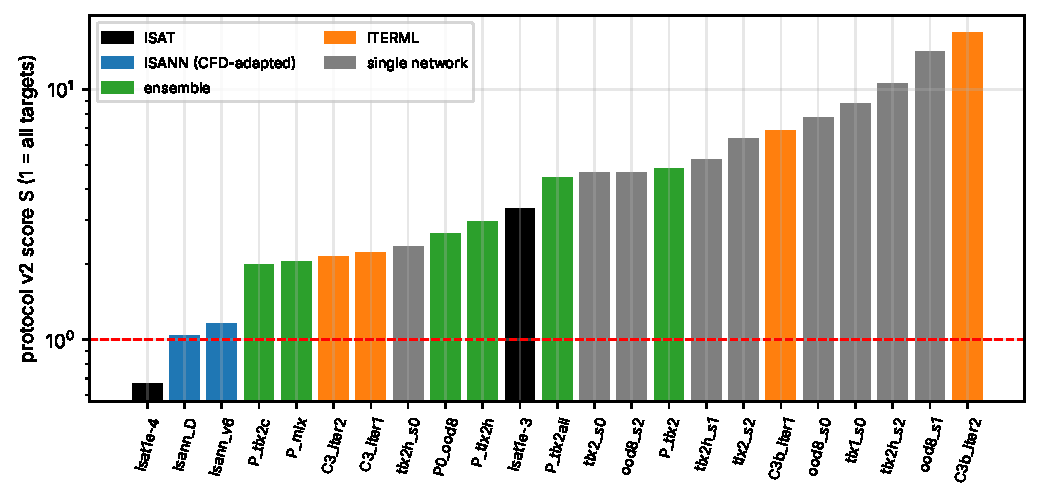
\includegraphics[width=\textwidth]{figs/fig_scores.pdf}
\caption{Protocol v2 score of every valid run (log scale); dashed red: $S=1$, every target met.}
\label{fig:scores}
\end{figure}

\begin{table}[t]
\centering
\caption{Selected protocol v2 results (pure mode, 4 ranks). Full list in \texttt{scores\_v2.csv}.}
\label{tab:scores}
\small
\resizebox{\textwidth}{!}{%
\begin{tabular}{llccccccc}
\toprule
Treatment & kind & $S$ & flame $|dT|$ [K] & ignition [ms] & $C$ & drift [K/10 ms] & OH L1 & s/step \\
\midrule
ISAT tol.\ \num{e-4}     & tabulation          & \textbf{0.67} & 0.9  & $-0.2$ & 0.01 & $+0.2$ & 0.8\%  & 3.65 \\
isann\_D                 & CFD-adapted network & 1.04 & 5.2  & $-0.2$ & 0.15 & $+0.4$ & 3.1\%  & 1.94 \\
isann\_v6                & CFD-adapted network & 1.16 & 5.8  & $-0.2$ & 0.22 & $+0.2$ & 11\%   & 2.09 \\
P\_tix2c                 & ensemble of 3       & 2.00 & 8.0  & $-0.6$ & 0.15 & $+0.5$ & 10\%   & 3.66 \\
P\_mix                   & ensemble of 6       & 2.05 & 10.3 & $-0.6$ & 0.50 & $+0.5$ & 19\%   & 7.12 \\
tix2h\_s0                & single network      & 2.35 & 11.8 & $+0.6$ & 1.34 & $+0.3$ & 32\%   & 1.99 \\
P0\_ood8                 & ensemble of 3       & 2.67 & 7.8  & $-0.8$ & 0.48 & $+0.1$ & 18\%   & 4.09 \\
ISAT tol.\ \num{e-3}     & tabulation          & 3.33 & 2.9  & $-1.0$ & 0.03 & $+0.5$ & 2.6\%  & 2.96 \\
ood8\_s1                 & single network      & 14.1 & 70.7 & $-1.0$ & 1.81 & $+10.8$ & 55\%  & 1.83 \\
\midrule
GA18 DI                  & reference           & 0    & 0    & 0      & 0    & 0      & 0      & 13.6 \\
\bottomrule
\end{tabular}}
\end{table}

\subsection{The reference line}
ISAT at tolerance \num{e-4} meets every target ($S=0.67$): 0.9~K in the flame, ignition 0.2~ms early, OH and CO
L1 errors below 1\%, at 3.65~s per step against 13.6~s for DI. Its table settles in under 1~ms of simulated time
(about 2900 leaves over four ranks, 89--90\% retrieves) and its cost then stays flat. At tolerance \num{e-3} it is
equally good in the flame (2.9~K) but ignites 1.0~ms early ($S=3.33$). No network meets every target; the best
CFD-adapted network is at $S=1.04$ and the best physics-only one at 2.00 (Fig.~\ref{fig:scores},
Table~\ref{tab:scores}). Without the ISAT line these networks would read as successes; with it, a network on this
18-species mechanism must reach ISAT's accuracy at a lower cost to be worth its training, and none does. The flow
and radiation solve alone costs 1.3~s per step, which caps any chemistry method at about a tenfold speed-up of the
whole step; a cold-cell cutoff saves only 8\% because the cost sits in the 14.6k hot cells.

\subsection{Training repeats and ensembles}
\label{sec:repeats}
Three repeats of the same recipe and data, differing only in the random seed of training, gave $S$ = 4.67, 7.72
and 14.1 (ood8), 2.35, 5.26 and 10.6 (tix2h), and 4.64 and 6.35 with one crash (tix2) (Fig.~\ref{fig:repeats}).
The spread within a family is larger than the differences between families; by an elitism rule that requires
every repeat of a candidate to beat the incumbent, no family beats another. A single-seed ranking of surrogates is
therefore noise on this case, and we expect the same elsewhere. The mean ensemble of the repeats beats its family
mean every time and stabilises every member (the crashing tix2 repeat ran to the end inside its ensemble), at about
1~s per step per member.

\begin{figure}[t]
\centering
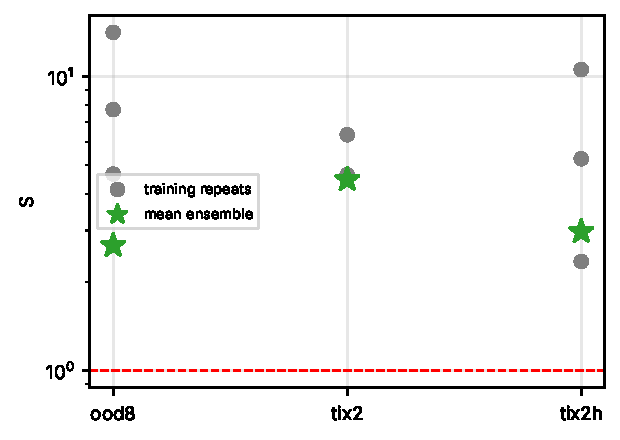
\includegraphics[width=0.55\textwidth]{figs/fig_repeats.pdf}
\caption{Protocol score of three training repeats per family (dots; one tix2 repeat crashed) and of their mean
ensemble (stars).}
\label{fig:repeats}
\end{figure}

\subsection{Ignition separates methods}
Most treatments fail on one term only, and that term is usually the ignition delay: ISAT \num{e-3}, the 6-member
ensemble and every physics-only family but one ignite the jet 0.2--1.4~ms early while their flame error is
moderate. The delay is set by the induction chemistry of a few cells at the jet base, which carry no weight in a
volume-averaged flame error and are invisible once the flame is established. A protocol with a flame window only
would rank ISAT \num{e-3} second of 25.

\subsection{Hybrid mode hides errors}
\label{sec:hybrid}
On the earlier configuration (protocol v1), the same a priori network kept the flame within 3.5--5.7~K in hybrid
mode, with about 1\% of the hot cells sent to DI, and was 68.8~K off and drifting by $+20$~K per 10~ms in pure mode.
The 1\% of DI cells sat where the network pumps radicals into hot lean gas, and correcting them every step was
enough to keep the flame right. Hybrid scores measure the network plus a DI corrector, not the network.

%% ===============================================================================================
\section{Do cheaper tests predict the protocol?}
\label{sec:cheap}

\subsection{Offline benchmark}
The offline benchmark advances 218 canonical states built with Cantera from the inlet streams (equilibrium,
cooled products, lean hot gas, vitiated mixtures, partially burnt mixtures, flamelet points; no CFD state) for
2500 steps of \SI{2e-5}{s} in homogeneous constant-$(p,h)$ reactors, with the surrogate alone and in a hybrid mode,
and reports one-step increment errors, radical errors at 1 and 10~ms, equilibrium fixed-point errors,
temperature errors at 1, 10 and 50~ms and the share of states drifting by more than 100~K. Over the 20 treatments
with a valid protocol score and a model file, none of its 33 metrics correlates significantly with $S$
(Fig.~\ref{fig:offline}): the best is the hybrid temperature error at 10~ms ($\rho=+0.36$, $p=0.12$), the composite
offline score reaches $\rho=+0.24$. The ignition term is the exception: the OH error at the equilibrium fixed point
($\rho=+0.59$, $p=0.007$) and the share of states flagged OOD at the start ($\rho=+0.56$) track $|I|$. On protocol v1
the same benchmark gave $\rho=0.28$--0.68 depending on the state set, and it ranked an iterative-loop network clearly
better than its predecessor (22.9 vs 31.8~K at 10~ms) that was clearly worse in the burner. What the offline
benchmark does reliably is reject very bad models (a neural ODE surrogate was last in both).

\begin{figure}[t]
\centering
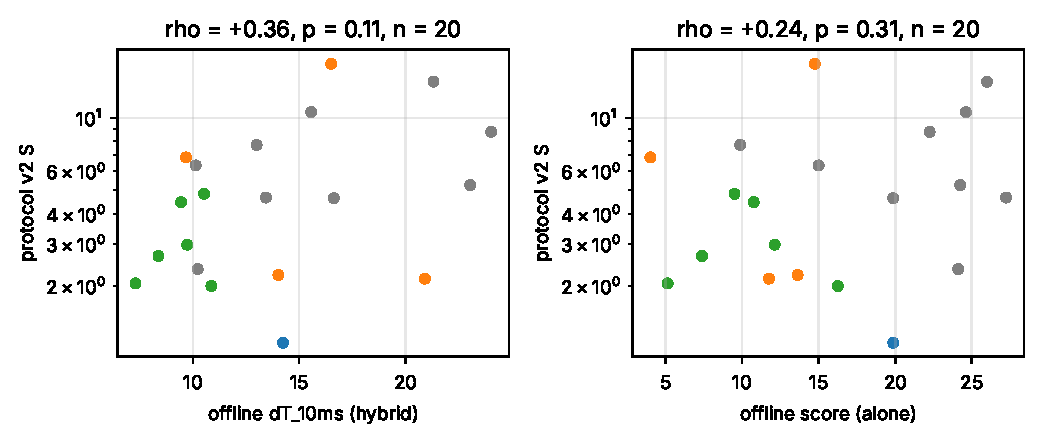
\includegraphics[width=\textwidth]{figs/fig_offline_vs_cfd.pdf}
\caption{Offline benchmark against protocol score, 20 treatments. Left: the best single offline metric; right: the
composite offline score. Colours as in Fig.~\ref{fig:scores}.}
\label{fig:offline}
\end{figure}

\subsection{One-step and shadow errors}
One-step errors are worse still as predictors. An online-trained network whose held-out one-step temperature error was
18 times lower than its predecessor's drifted by $-60$ to $-110$~K in 100-step 0D rollouts of cooled lean gas and had
to be rejected. Shadow checks in the burner show one-step temperature errors of 0.02--0.05~K for networks whose
flame errors range from 5 to 35~K: errors that are small per step and coherent over many steps build up below any
one-step threshold.

\subsection{A shorter flame window}
The flame error at 10 or 20~ms into the flame phase, combined with the ignition and species terms, ranks the 23 valid
runs with $\rho=0.63$ and 0.65 against the full score ($p<0.002$), and for 20 of them it is within 20\% of the full
$S$. The two exceptions are the most instructive results of the study: two ITERML ensembles trained from scratch had
1.7--3.7~K flame errors at 20~ms (they would have scored 0.44 and 1.33, the first apparently meeting every target),
then drifted in the rich core under the nozzle from 25~ms on and ended at $S=6.86$ and 16.8. Every repeat had passed
the offline gate. A short window is a good screen, but acceptance needs the full window, and a longer one would be
safer.

\subsection{A steady reference}
A steady local-time-stepping DI solution with wall radiation passes the same gate G1 as the transient flame reference
(hot volume 19.62 vs 18.25~cm$^3$, mean hot-cell difference 47.6~K vs Fluent) after 17.6~h on eight cores. A steady
flame phase scored against it could replace the 50~ms transient for a cheaper screen of the established flame
\todo{not yet tested with surrogates}.

%% ===============================================================================================
\section{Discussion and recommendations}
\label{sec:discussion}
The protocol costs about 2.7~h per candidate on four cores, far more than an offline benchmark (3~min) but small
against the cost of training a candidate (3--18~h here). Every shortcut we tried mispredicts it in a way that matters:
offline and one-step errors do not rank candidates; hybrid scores hide the network's errors; a flame-only window
ignores ignition; a short window misses slow coupled drift; a single training seed is not a sample. We therefore
recommend, for any paper that proposes a chemistry surrogate for CFD:
\begin{enumerate}
\item validate the DI reference first, against an independent solver or experiment;
\item run the surrogate in pure mode;
\item score an ignition (or other transient) phase and the established flame separately, and combine them with a
  maximum so that no term can hide another;
\item report several training repeats, or a mean ensemble, never a single seed;
\item run a tabulation method (ISAT) at the same ranks and report the cost per step with the chemistry share;
\item keep shadow-DI comparison data with every run, and version the settings.
\end{enumerate}

\paragraph{Limitations} One laminar burner, one mechanism and one fuel; one solver. The targets (5~K, 0.3~ms, factor
1.4) are choices for this case. The protocol needs a validated DI reference, which for large mechanisms or turbulent
cases is expensive. \todo{Port the protocol to the Fluent case (pure mode is its only mode).}

\subsection{History: protocol v1}
\label{sec:history}
Version 1 was run on an earlier configuration of the burner (lateral side open, top and chimney closed, no wall
radiation, unity-Schmidt species diffusion) from one lit start, scored the start-up (0--5~ms) and the flame
(25--50~ms) separately and had no single score. Its results showed the masking by hybrid mode and the poor offline
correlation reported above; the corrections of the case (outlets, radiation, diffusion) and the codified score of
version 2 came from them.

\section{Conclusions}
A fixed CFD protocol in pure mode, with an ignition phase, a flame phase and one score, separates chemistry treatments
that offline tests cannot: on a laminar methane/air burner only ISAT at tolerance \num{e-4} met every target, training
repeats of one network spanned a factor of 2--5 in score, the ignition delay decided most rankings, and no offline
metric predicted the protocol's order. Surrogate papers should be judged in the solver, in pure mode, against a
validated reference and a tabulation baseline.

\section*{Data and code availability}
\todo{openfoam/protocol (protocol\_v2\_ign.yaml, protocol\_v2\_flame.yaml, run\_protocol\_v2.sh, score\_v2.py),
openfoam/iterml/rules.py, scripts/18\_offline\_benchmark.py, results/sim1/.}

\section*{Acknowledgements}
\todo{}

\bibliographystyle{elsarticle-num}
\bibliography{refs}

\end{document}
